%Este trabalho está licenciado sob a Licença Atribuição-CompartilhaIgual 4.0 Internacional Creative Commons. Para visualizar uma cópia desta licença, visite http://creativecommons.org/licenses/by-sa/4.0/deed.pt_BR ou mande uma carta para Creative Commons, PO Box 1866, Mountain View, CA 94042, USA.

\chapter{Vetores}\label{cap_vetor}
\thispagestyle{fancy}

\section{Segmentos orientados}\label{cap_vetor_sec_segorien}

Sejam dois pontos $A$ e $B$ sobre uma reta $r$. O conjunto de todos os pontos de $r$ entre $A$ e $B$ é chamado de \pmb{segmento}\index{segmento} $AB$.

\begin{figure}[h!]
  \centering
  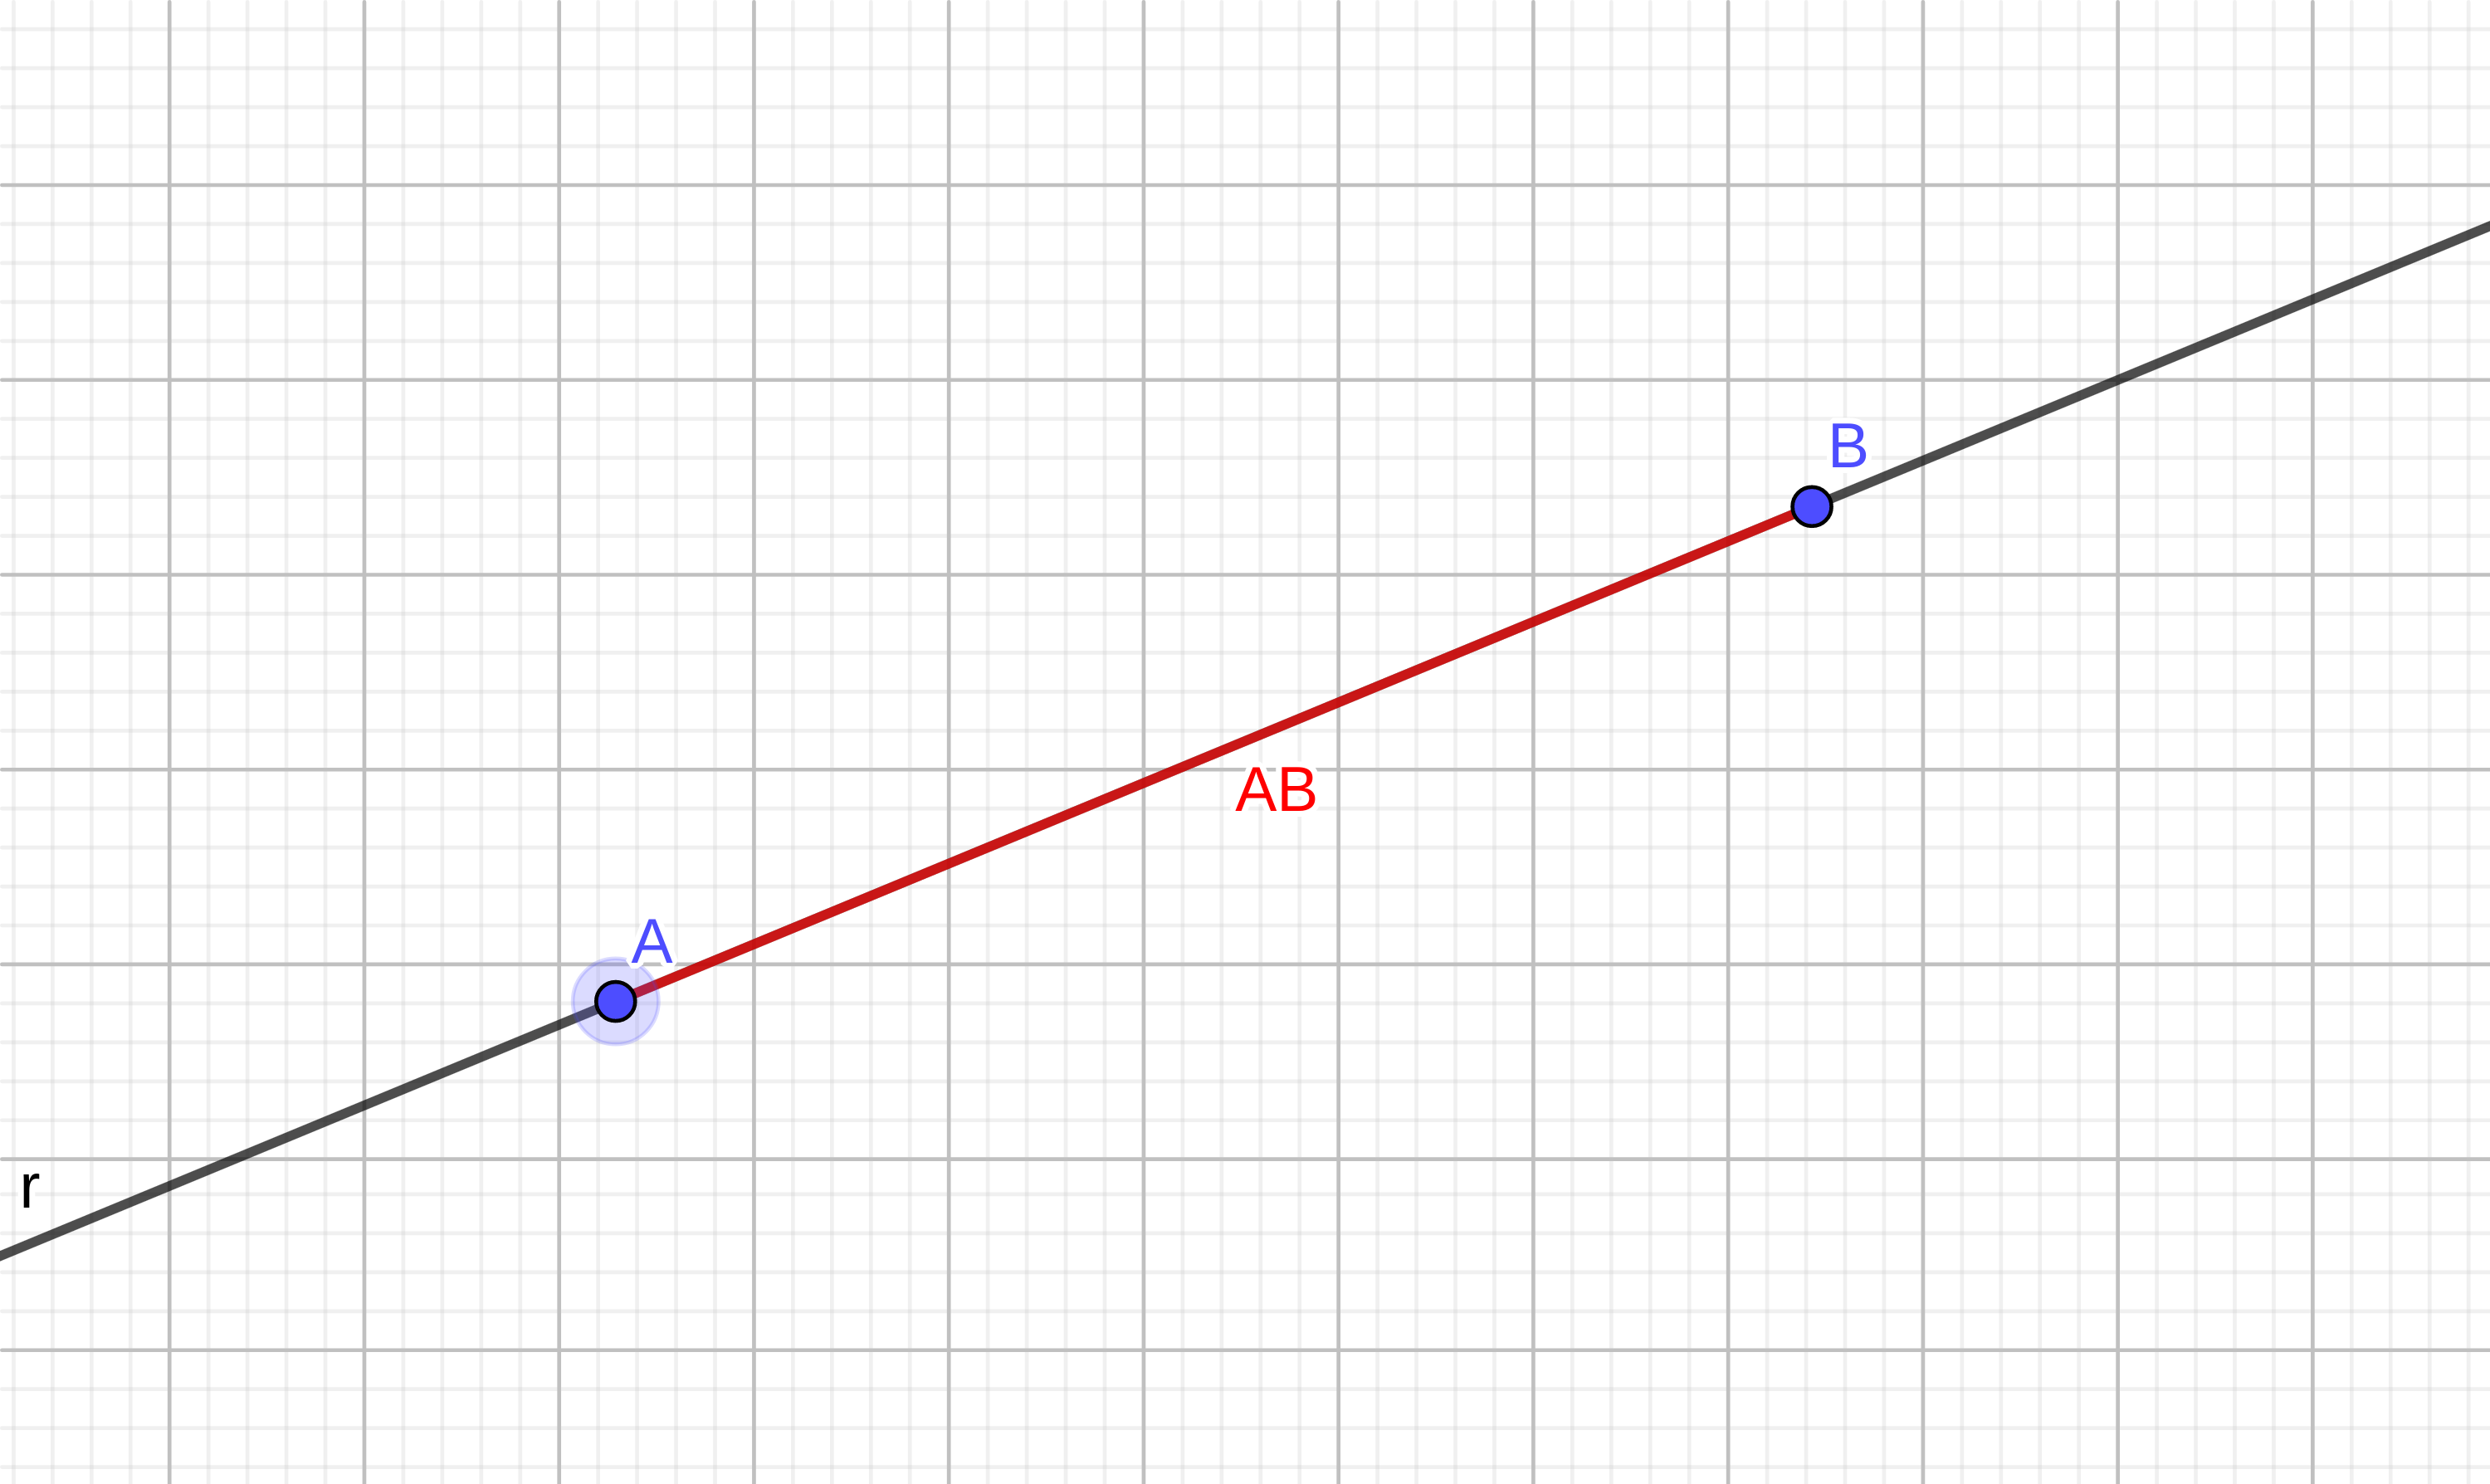
\includegraphics[width=0.7\textwidth]{./cap_vetor/dados/fig_segmento/fig_segmento}
  \caption{Esboço de um segmento $AB$.}
  \label{fig:segmento}
\end{figure}

Associado a um segmento $AB$, temos seu \pmb{comprimento}\index{comprimento} (ou tamanho), o qual é definido como sendo a \pmb{distância}\index{distância} entre os pontos $A$ e $B$. A distância entre os ponto $A$ e $B$ é denotada por $|AB|$ ou $|BA|$.

A \pmb{direção} de um segmento $AB$ é a direção da reta que fica determinada pelos pontos $A$ e $B$.

\begin{ex}\label{ex:segmento}
  Consideremos os segmentos esboçados na Figura \ref{fig:ex_segmento}. Os segmentos $AB$ e $CD$ têm as mesmas direções, mas comprimentos diferentes. Já, o segmento $EF$ tem direção diferente dos segmentos $AB$ e $CD$.
  
  \begin{figure}[h!]
    \centering
    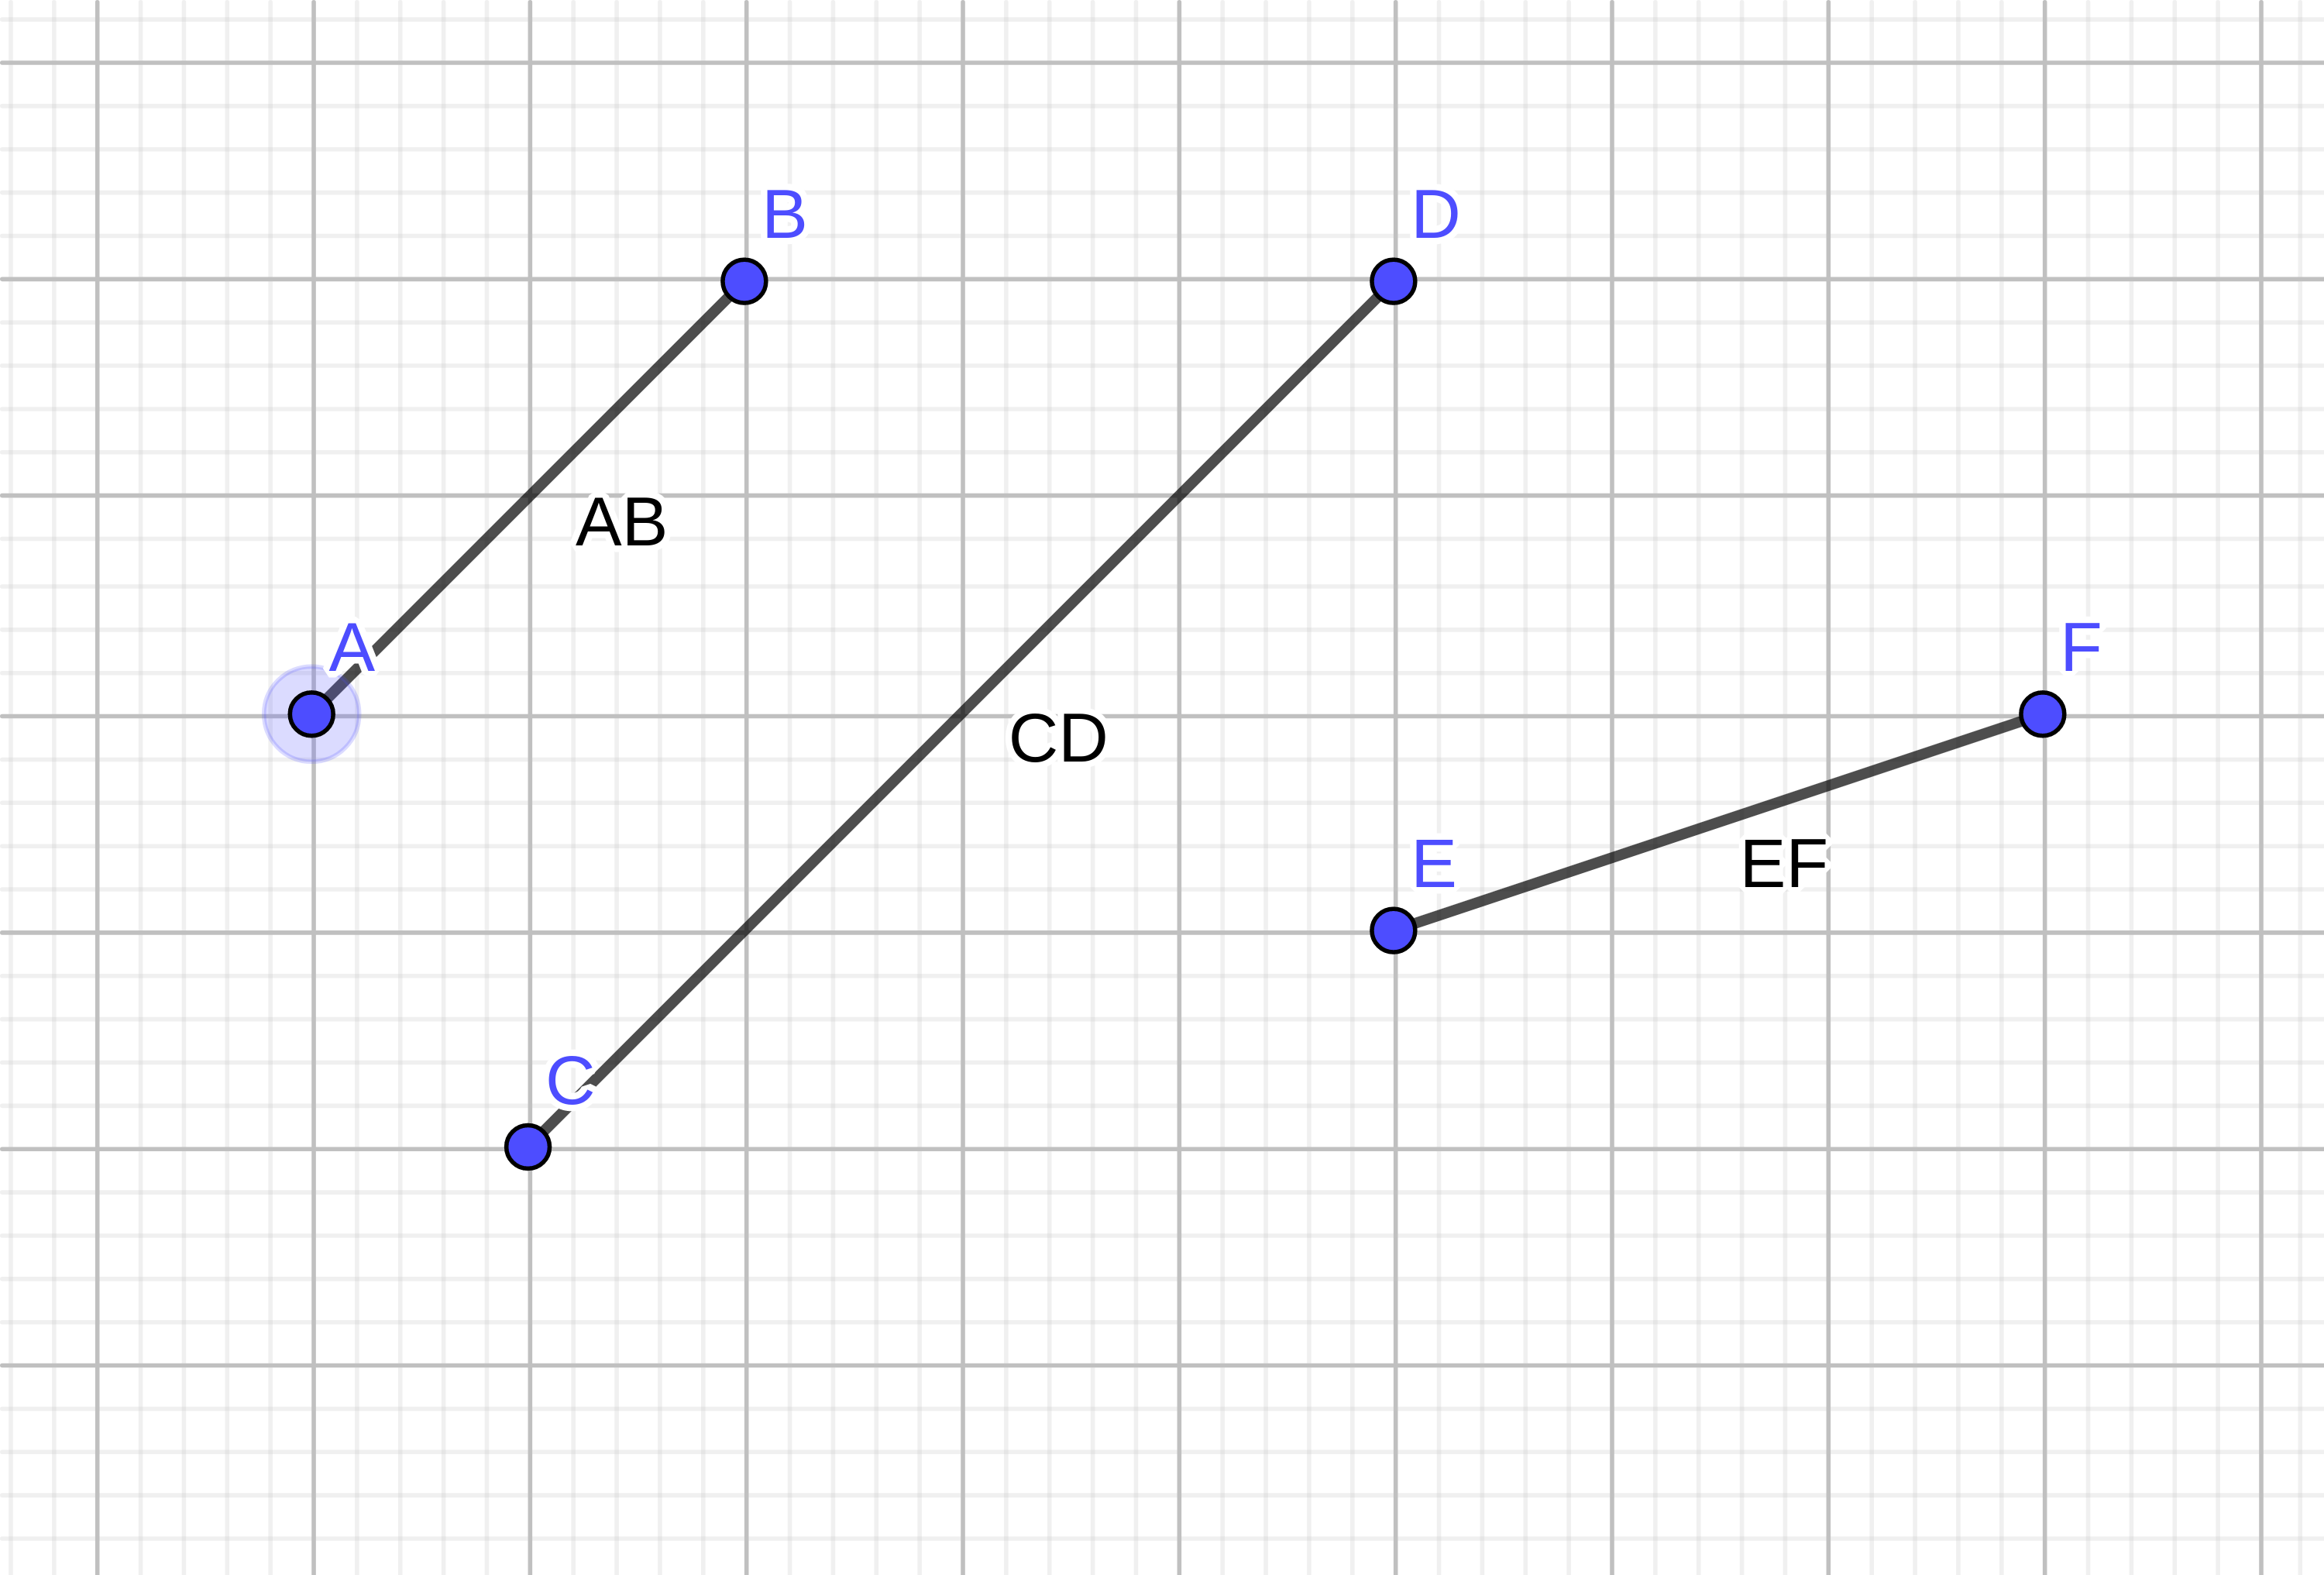
\includegraphics[width=0.7\textwidth]{./cap_vetor/dados/fig_ex_segmento/fig_ex_segmento}
  \caption{Esboço referente ao Exemplo \ref{ex:segmento}.}
  \label{fig:ex_segmento}
\end{figure}
\end{ex}

Se $A$ e $B$ são o mesmo ponto, então chamamos $AB$ de \pmb{segmento nulo}\index{segmento nulo} e temos $|AB| = 0$. Um segmento nulo não tem direção.

\begin{figure}[h!]
  \centering
  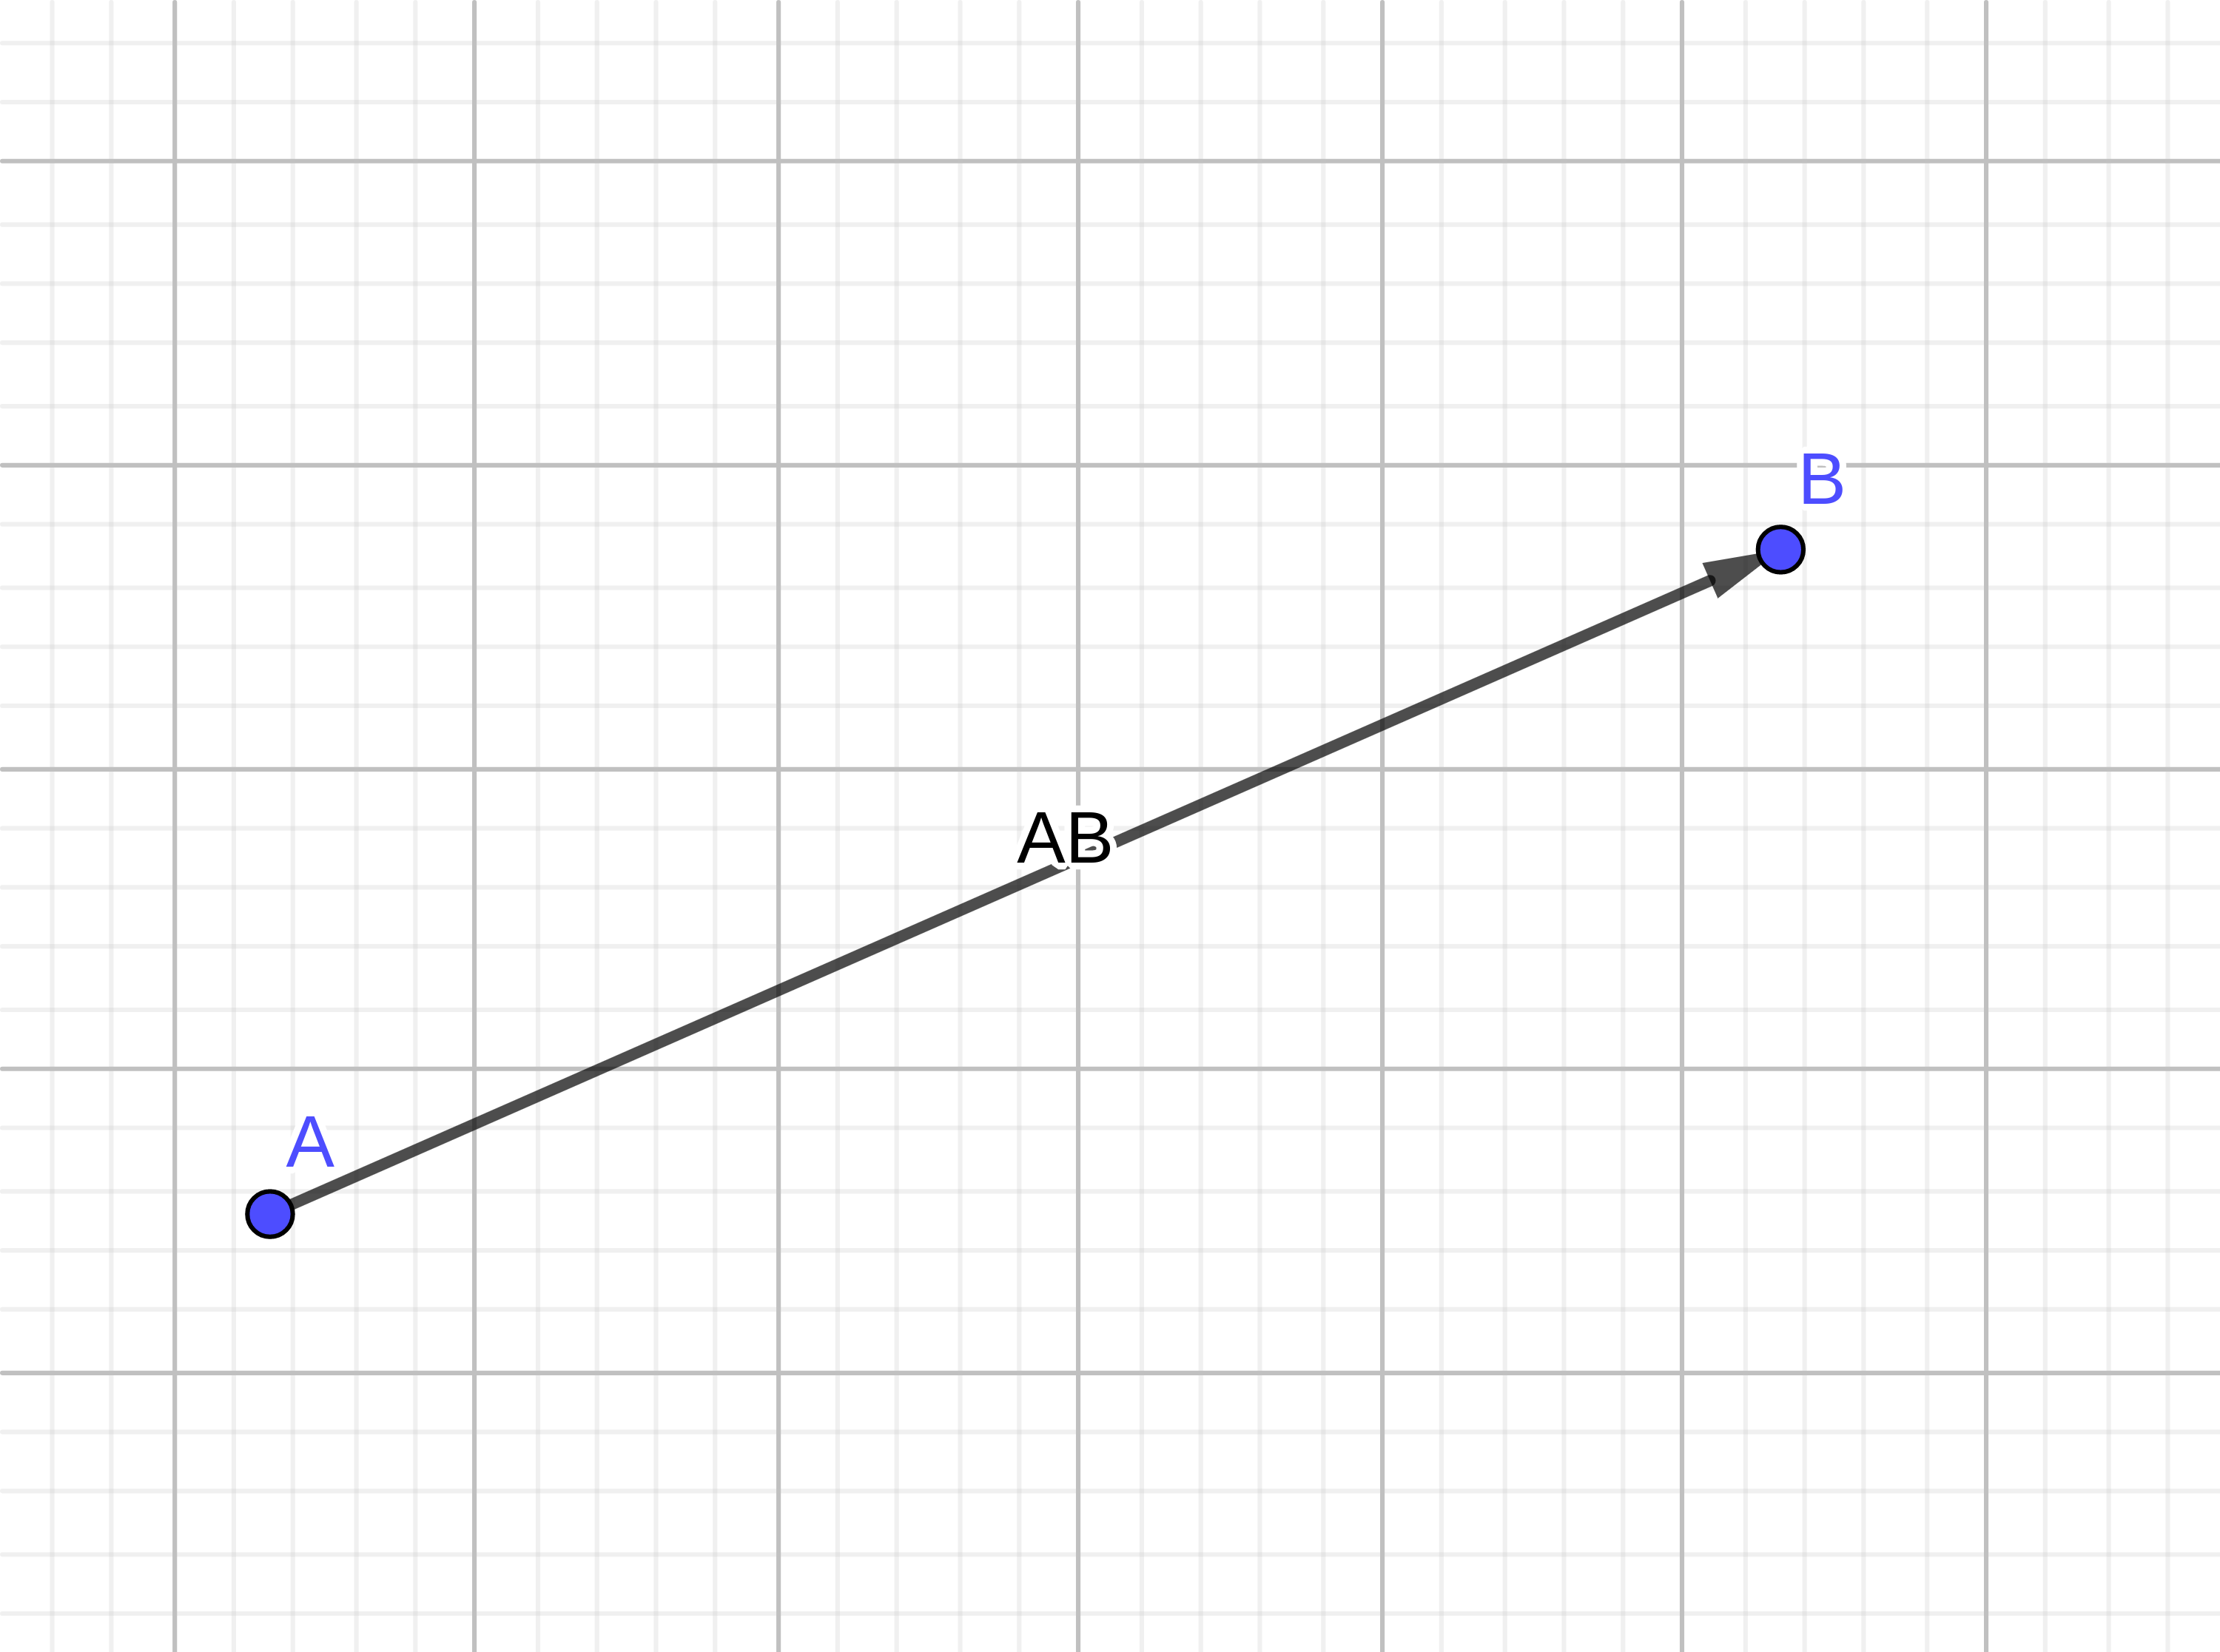
\includegraphics[width=0.7\textwidth]{./cap_vetor/dados/fig_seg_orientado/fig_seg_orientado}
  \caption{Esboço de um segmento orientado $AB$.}
  \label{fig:seg_orientado}
\end{figure}


Observemos que um dado segmento $AB$ é igual ao segmento $BA$. Agora, podemos associar a noção de \pmb{sentido} a um segmento, escolhendo um dos pontos como sua \pmb{origem}\index{origem} e o outro como sua \pmb{extremidade}\index{extremidade}. Ao fazermos isso, definimos um \pmb{segmento orientado}\index{segmento orientado}. Mais precisamente, um segmento orientado $AB$ é o segmento definido pelos pontos $A$ e $B$, sendo $A$ a origem e $B$ a extremidade. Veja a Figura \ref{fig:seg_orientado}.

Dizemos que dois dados segmentos orientados não nulos $AB$ e $CD$ têm a \pmb{mesma direção} quando as retas $AB$ e $CD$ forem paralelas ou coincidentes.

\begin{ex}\label{ex:segorien_direcao}
  Consideremos os segmentos orientados esboçados na Figura \ref{fig:ex_segorien_direcao}. Observemos que os segmentos orientados $AB$ e $CD$ têm a mesma direção. Já o segmento orientado $EF$ tem direção diferente dos segmentos $AB$ e $CD$.
  
  \begin{figure}[h!]
    \centering
    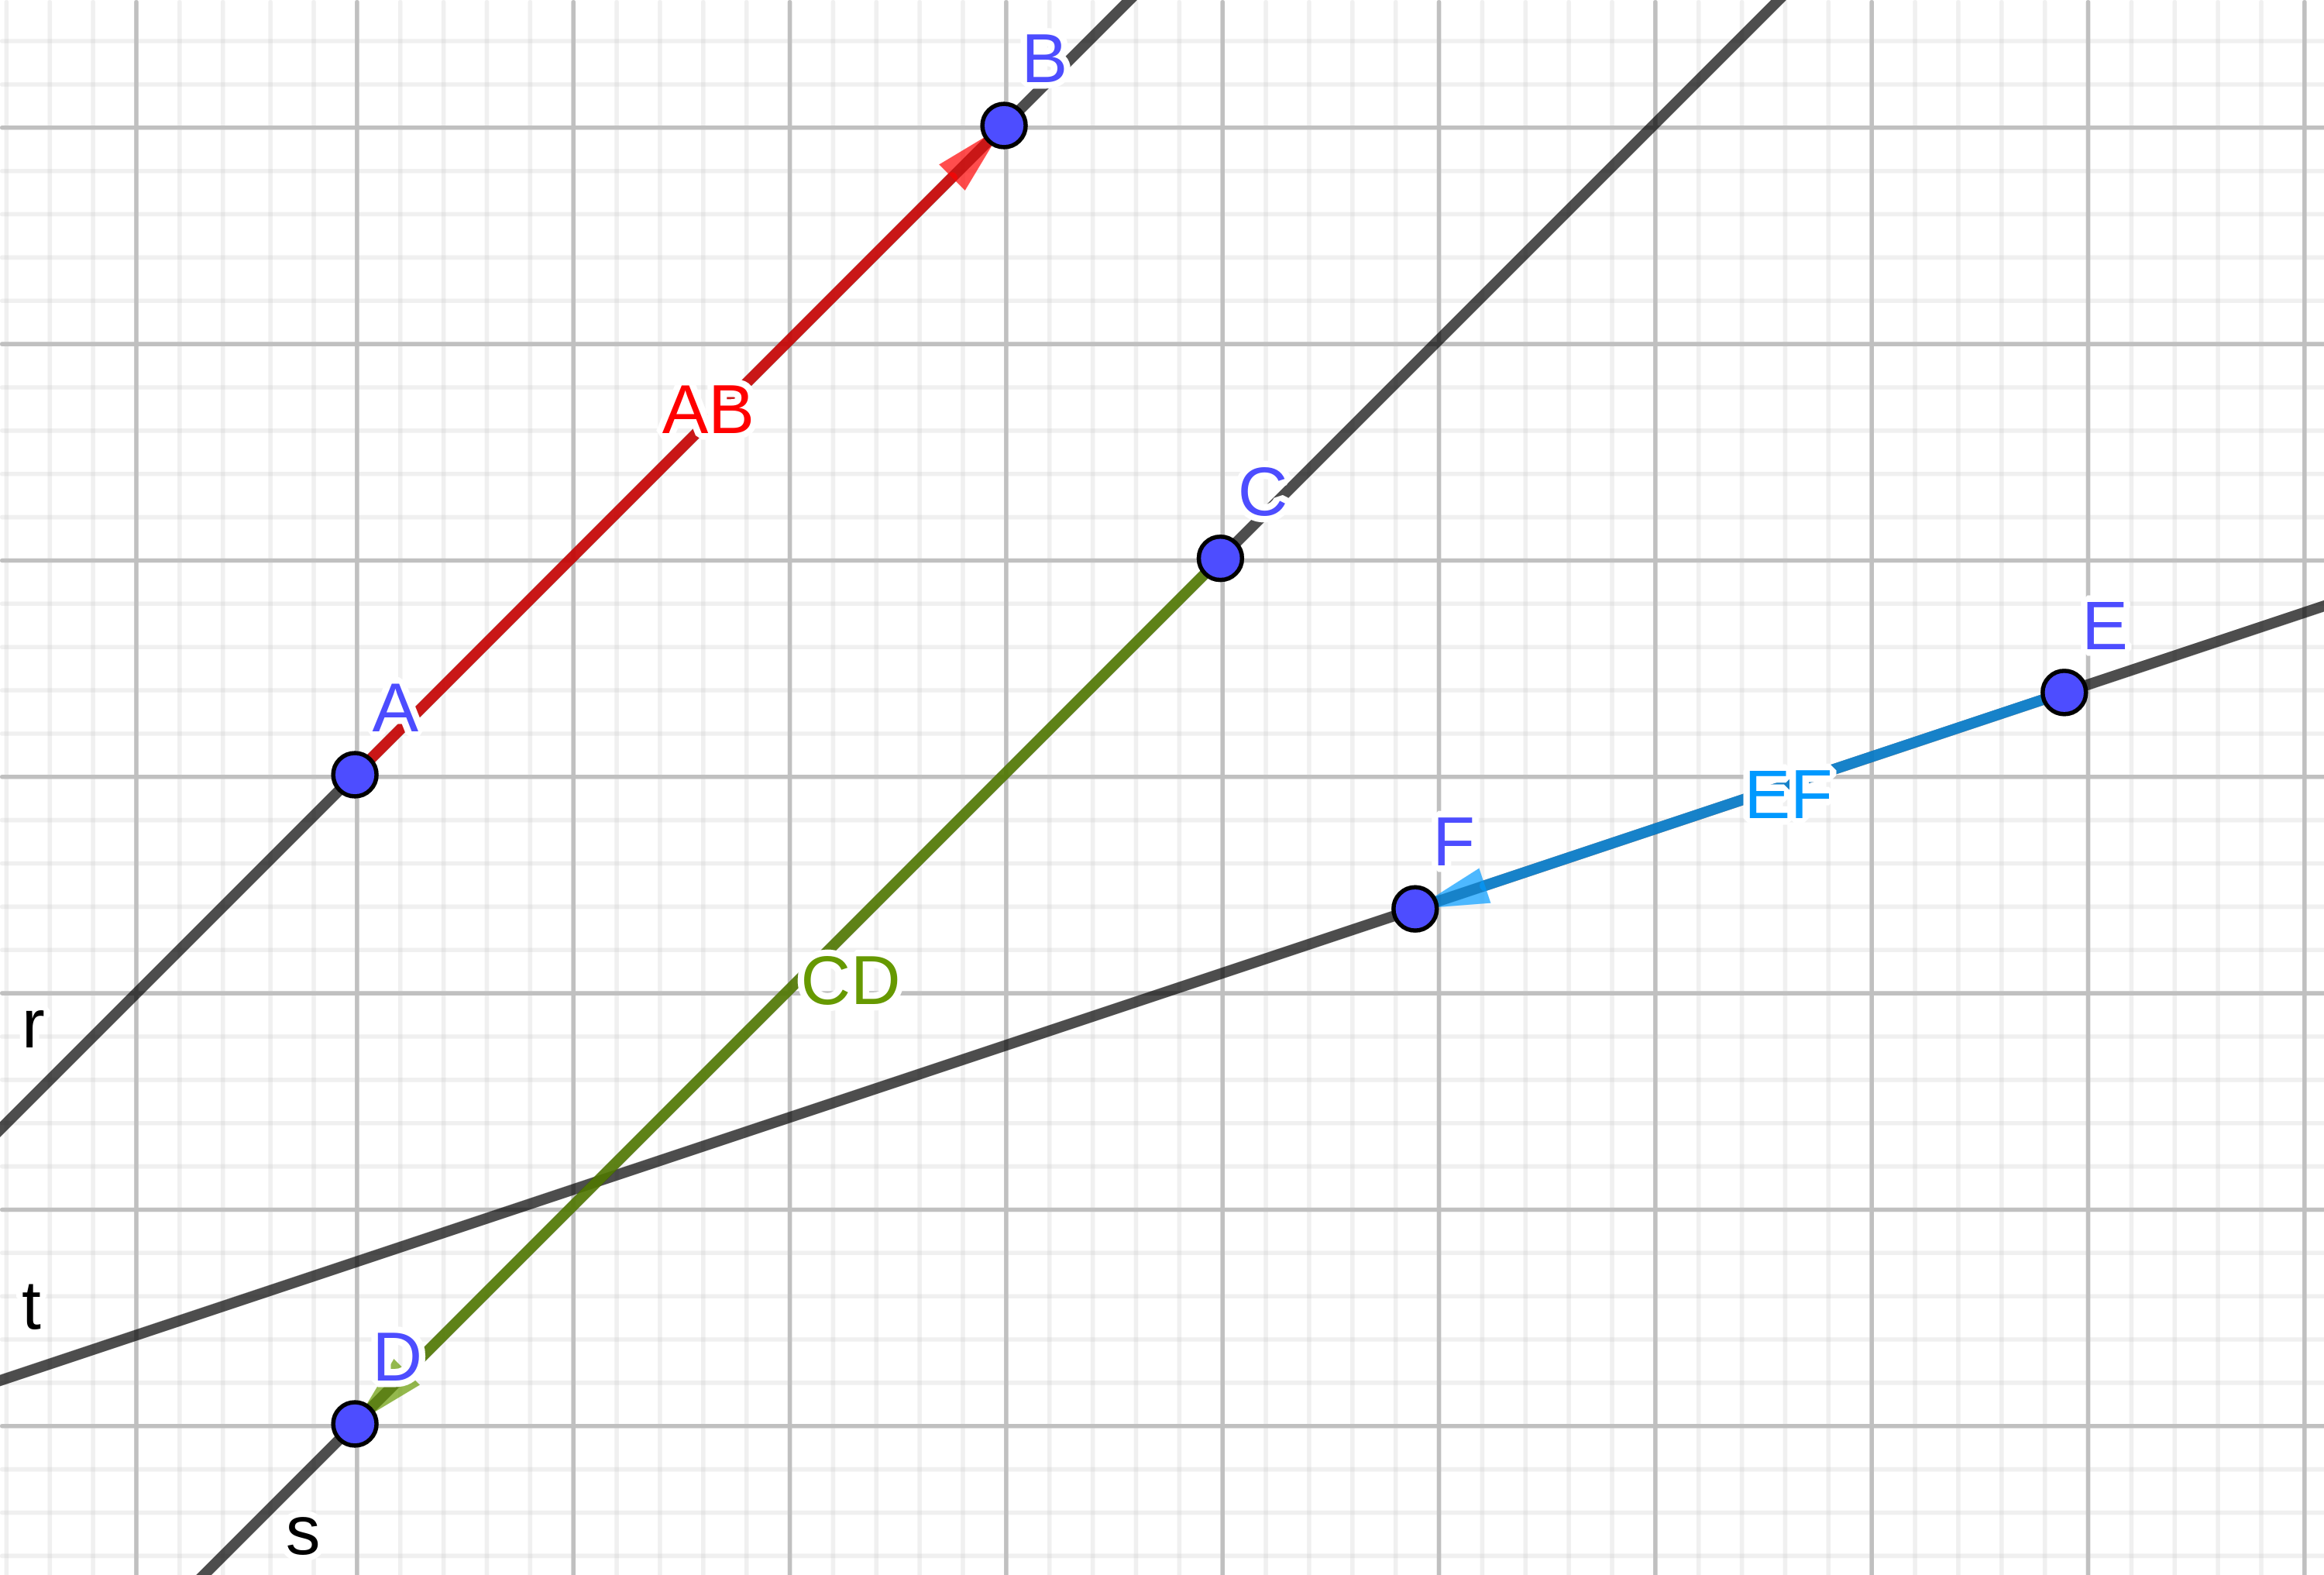
\includegraphics[width=0.7\textwidth]{./cap_vetor/dados/fig_ex_segorien_direcao/fig_ex_segorien_direcao}
  \caption{Esboço referente ao Exemplo \ref{ex:segorien_direcao}.}
  \label{fig:ex_segorien_direcao}
\end{figure}  
\end{ex}

Sejam dados dois segmentos orientados $AB$ e $CD$ de mesma direção, cujas retas $AB$ e $CD$ não sejam coincidentes. Então, as retas $AB$ e $CD$ determinam um único plano e a reta $AC$ determina dois semiplanos (veja a Figura \ref{fig:segorien_sentido}). Assim sendo, dizemos que os segmentos $AB$ e $CD$ têm \pmb{mesmo sentido}\index{mesmo sentido} quando os pontos $B$ e $D$ estão ambos sobre o mesmo semiplano.

\begin{figure}[h!]
  \centering
  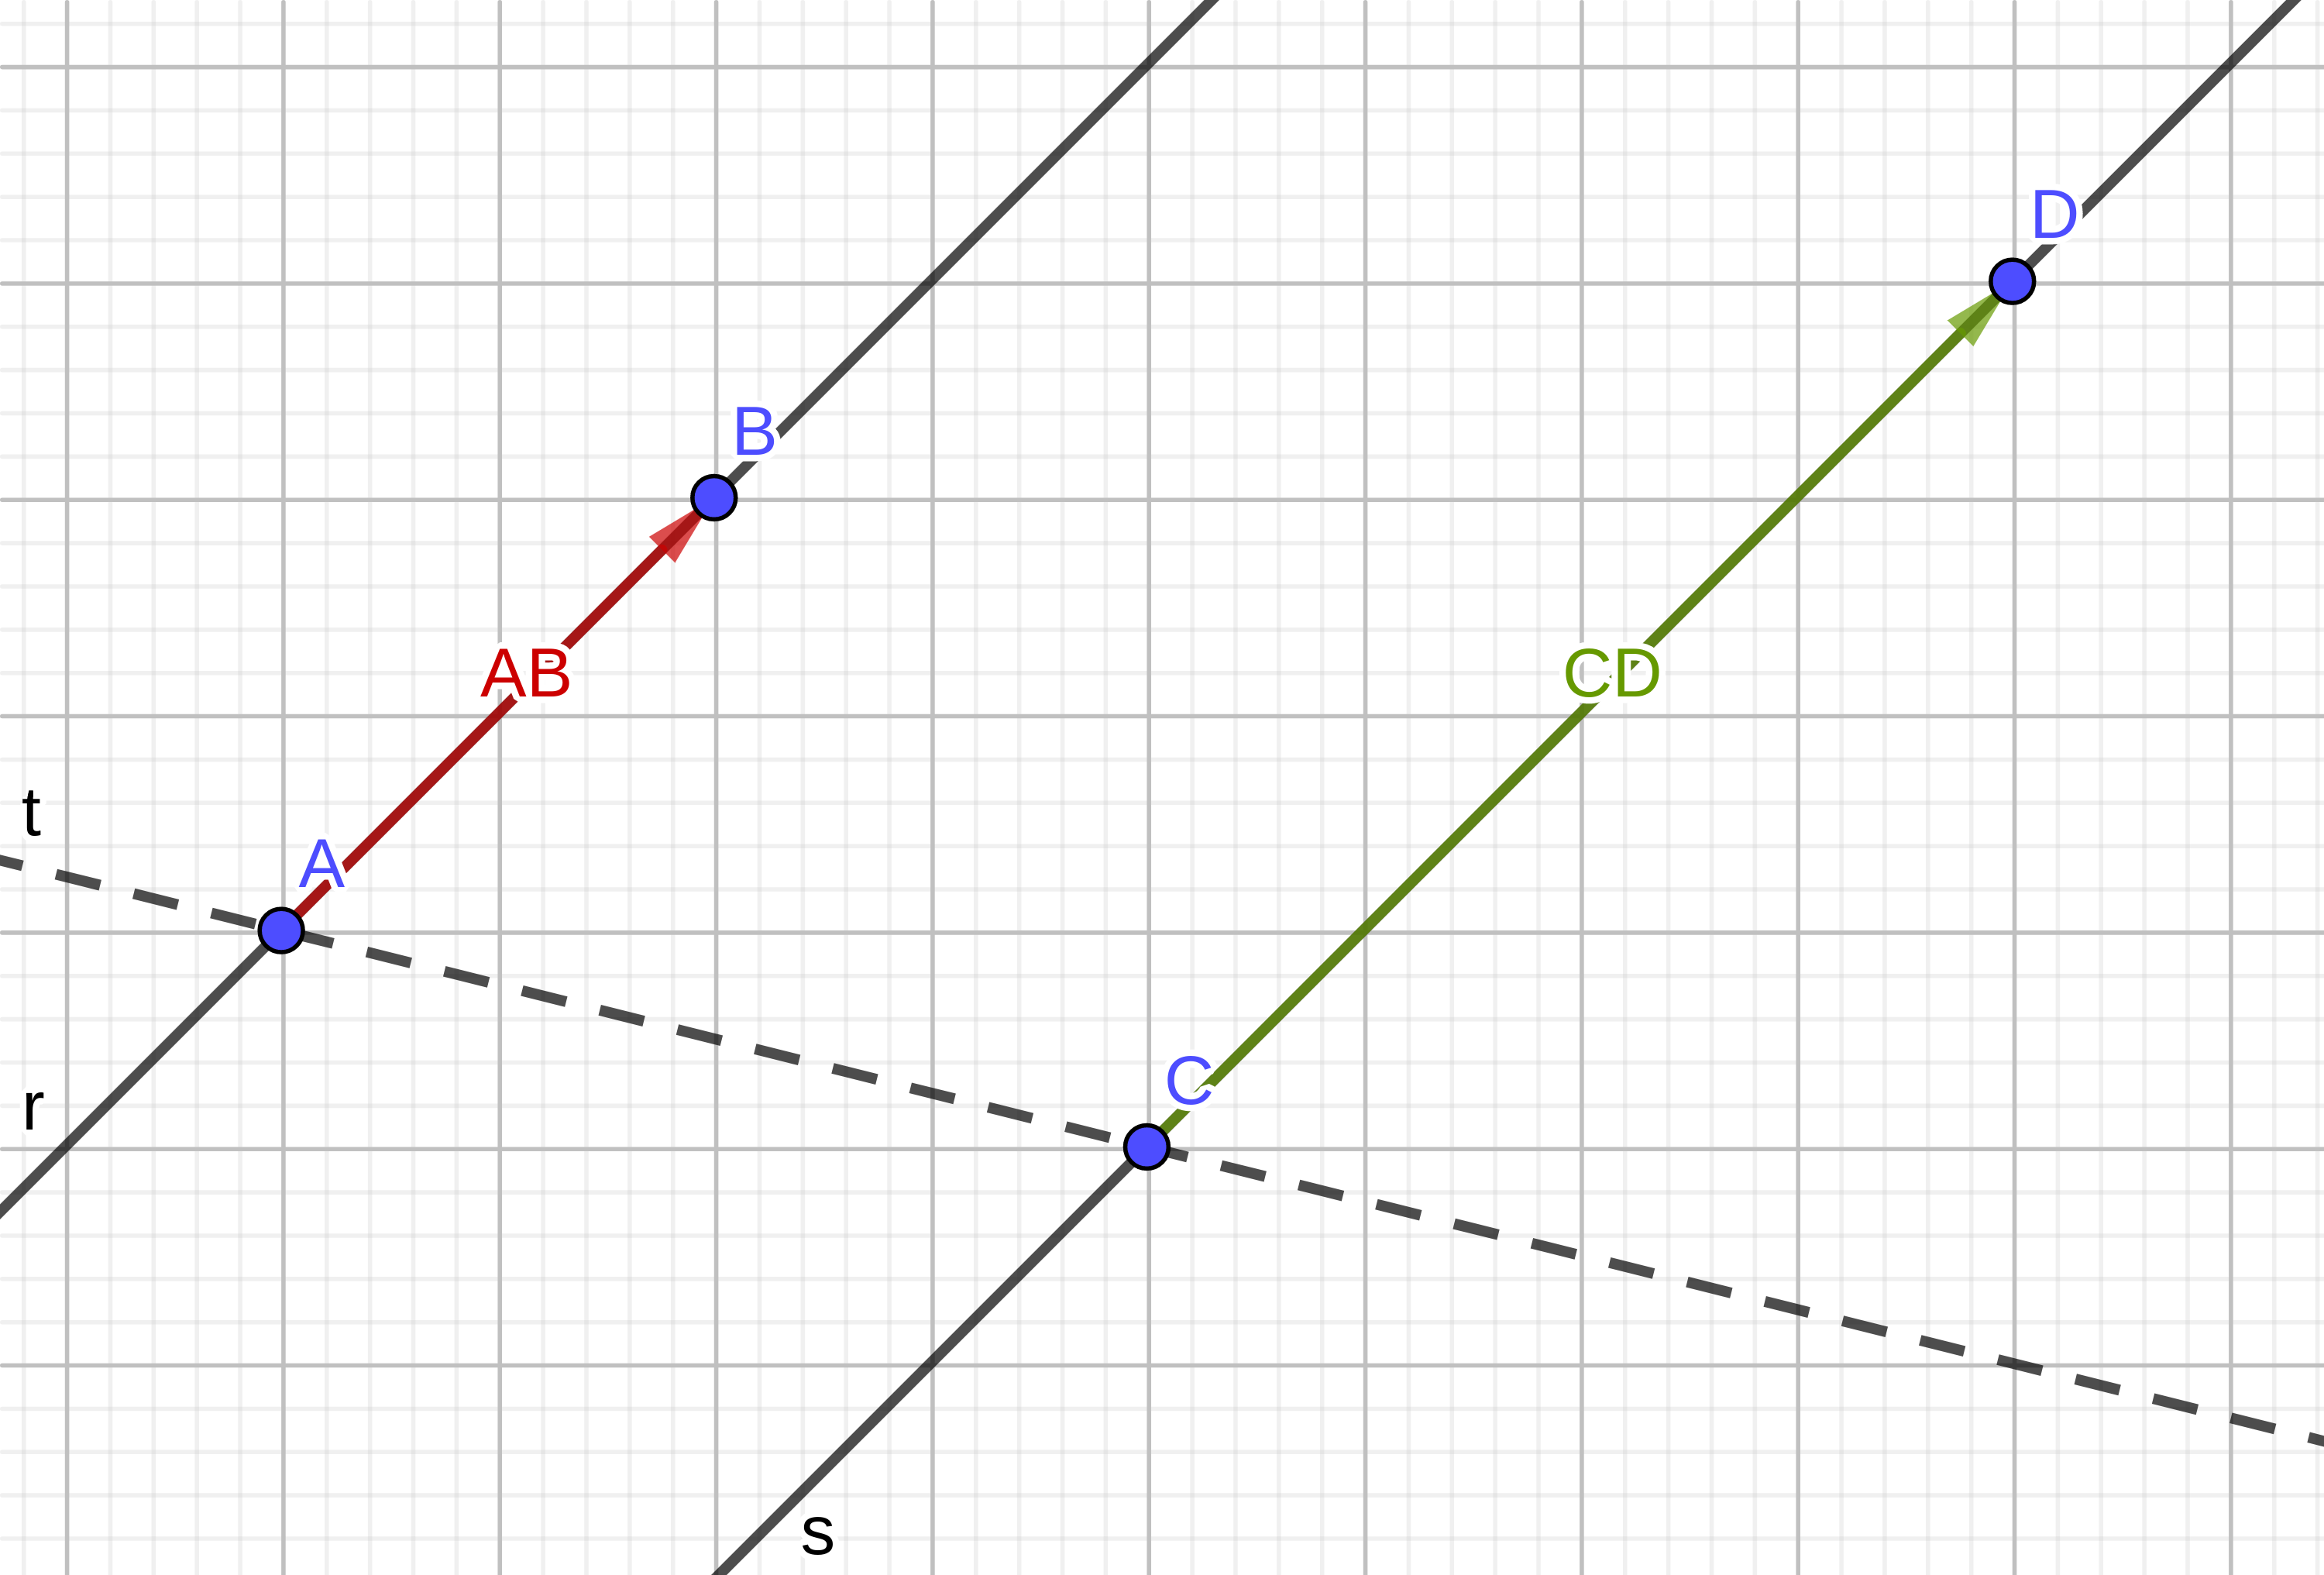
\includegraphics[width=0.7\textwidth]{./cap_vetor/dados/fig_segorien_sentido/fig_segorien_sentido}
  \caption{Esboço de dois segmentos orientados $AB$ e $CD$ de mesmo sentido.}
  \label{fig:seg_segorien_sentido}
\end{figure}

Para analisar o sentido de dois segmentos orientados e colineares, escolhemos um deles e construímos um segmento orientado de mesmo sentido a este, mas não colinear. Então, analisamos o sentido dos segmentos orientados originais com respeito ao introduzido.

\subsection{Exercícios}

\emconstrucao